\documentclass{beamer}
\usetheme{Madrid}
\usefonttheme{structurebold}
\title{Ask Me!}
\author{Softure - CPLUS}
\begin{document}
\maketitle
\begin{frame}
\frametitle{Introduction}
Ask me! app analyse social networks from different sources like twitter, facebook or foursquare to get important feedback about what a user searchs.
\end{frame}
\begin{frame}
\frametitle{Tools}
\begin{itemize}
\item C++ GNU
\item NodeJS
\item Javascript
\item HTML5
\item Netbeans
\end{itemize}
\end{frame}

\begin{frame}
\frametitle{Third Party Libraries}
\begin{itemize}
\item Porter Stemmer
\item FANN
\item Wordnet Blast
\item JsonCPP
\item Curl
\end{itemize}
\end{frame}

\begin{frame}
\frametitle{Sources}
\begin{itemize}
\item ConceptNet
\item Wordnet
\item Twitter
\item Foursquare
\item OpenStreetMap
\item Alchemy app
\end{itemize}
\end{frame}

\begin{frame}
\frametitle{Architecture}
\begin{center}
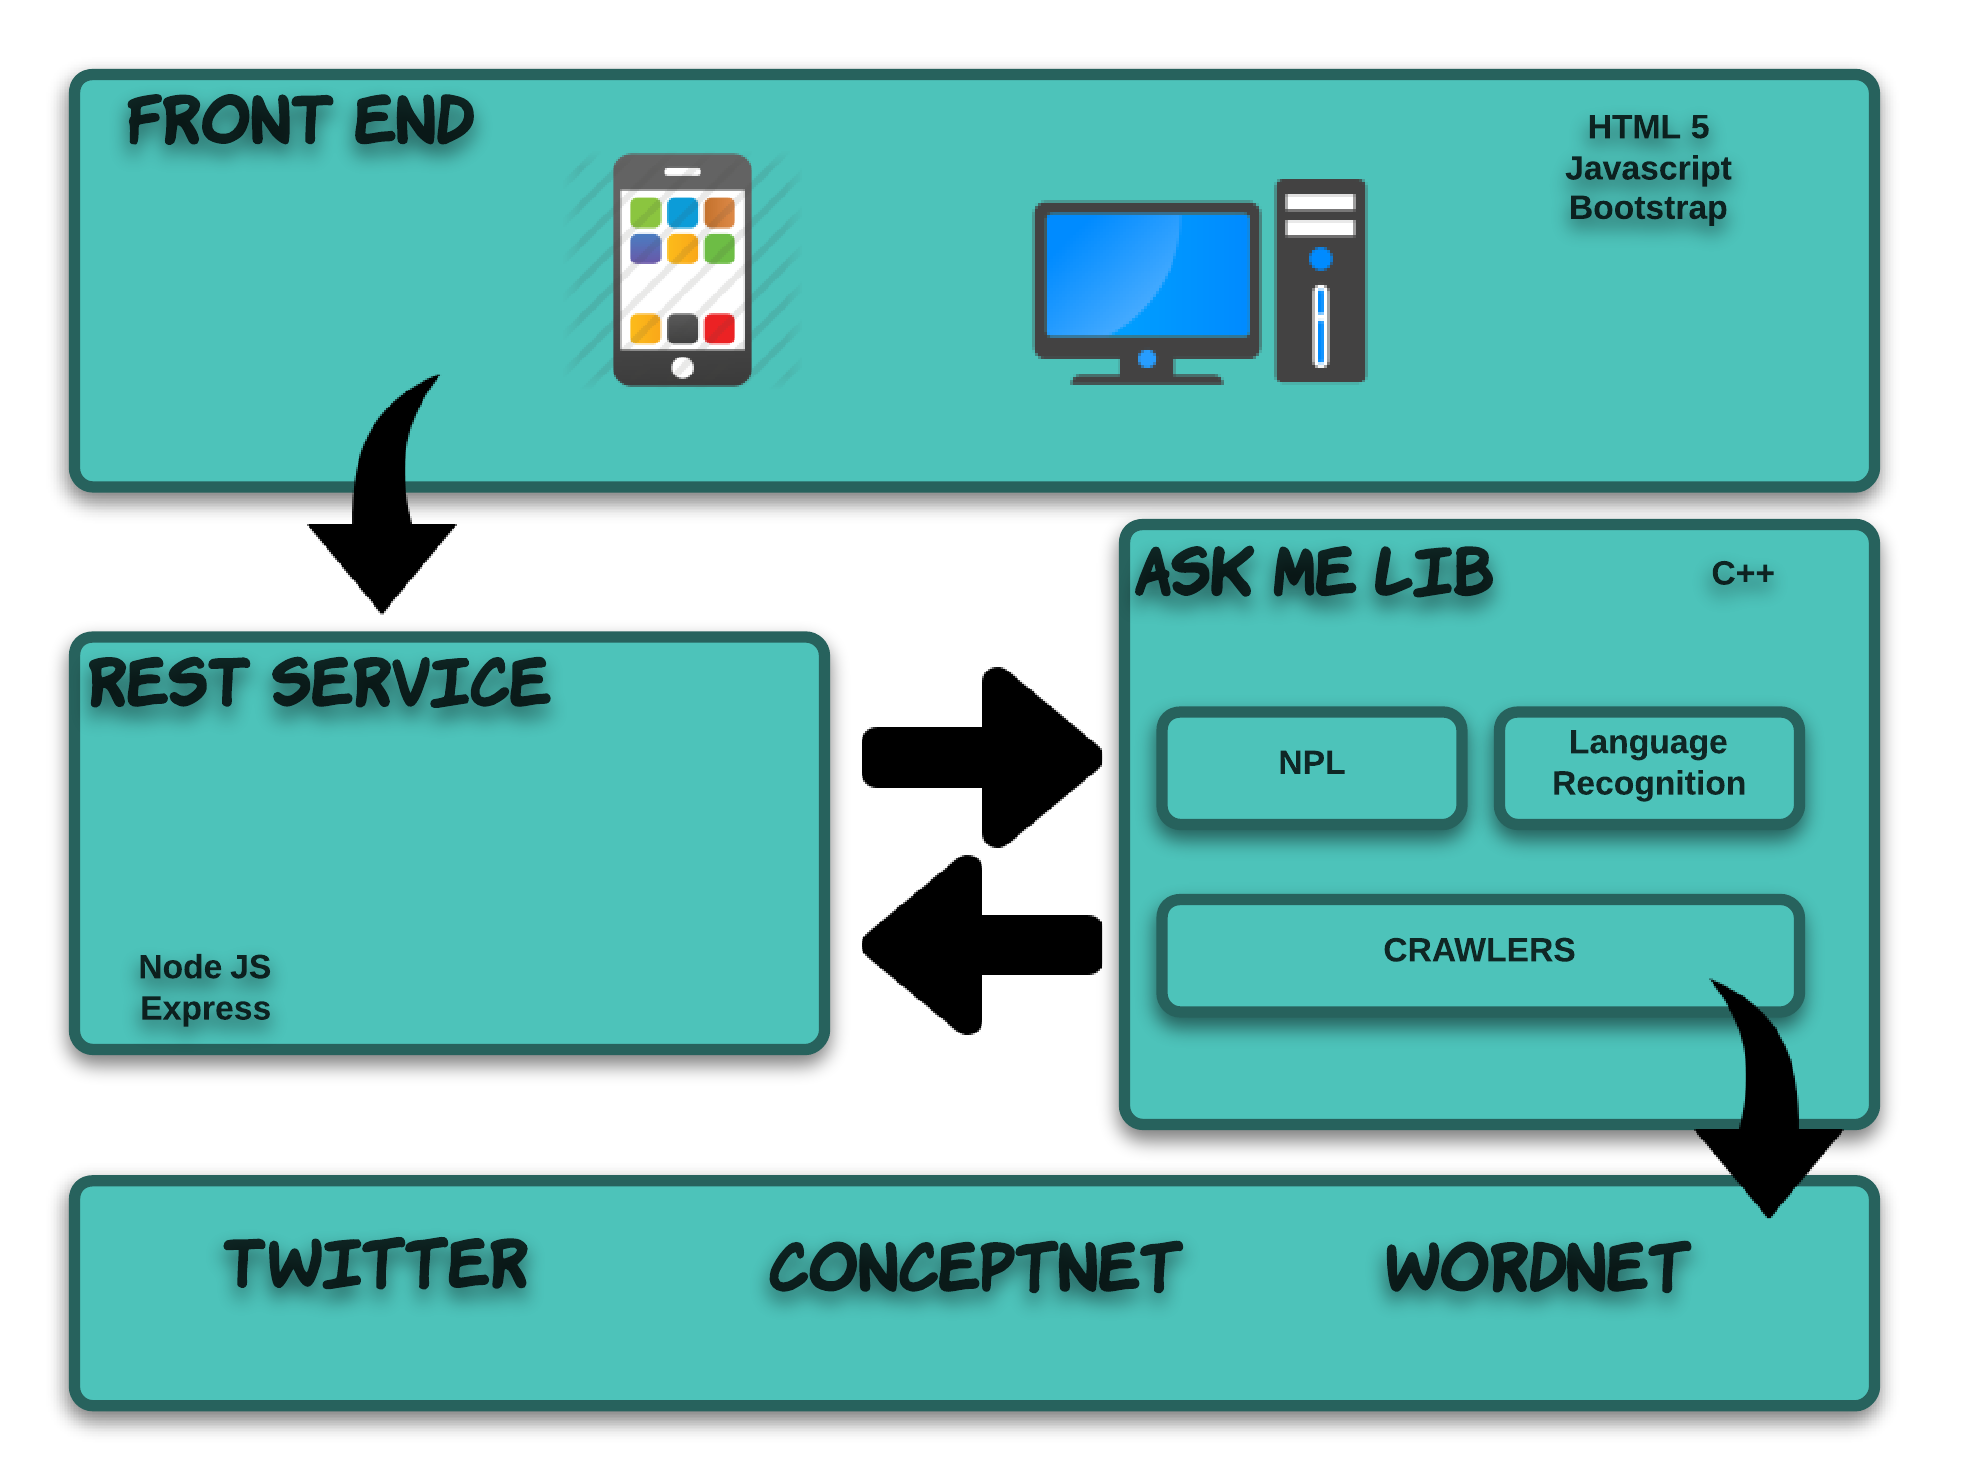
\includegraphics[height=3.0in]{AskMeArchitecture.png}
\end{center}
\end{frame}

\begin{frame}
\frametitle{Natural Language Processing}
It was identified some steps to achieve this task:
\begin{enumerate}
\item Define the language
\item Remove stop words
\item Apply stemming algorithm
\item Match with search parameters
\end{enumerate}
Also was performed this task to get other important information from obtained data:
\begin{enumerate}
\item Entity recognition
\item Sentiment analysis
\item Concept disambiguation
\end{enumerate}
\end{frame}

\begin{frame}
\begin{center}
DEMO
\end{center}
\end{frame}

\begin{frame}
\frametitle{Restrospective}
Bad
\begin{itemize}
\item Lack of commitment
\item Short time for a big field of knowledge
\item Use libraries already implemented instead of create them.
\end{itemize}
Good
\begin{itemize}
\item Research
\item New technologies
\end{itemize}
\end{frame}
\end{document}